\documentclass[11pt]{report}
% Same style as 1-foundations/theory/preamble.tex (the course's own documents).

\usepackage[a4paper,margin=2.3cm,headheight=14pt]{geometry}
\usepackage[T1]{fontenc}
\usepackage[utf8]{inputenc}
\usepackage{lmodern}
\usepackage{microtype}
\usepackage{booktabs}
\usepackage{longtable}
\usepackage{array}
\usepackage{xcolor}
\usepackage{enumitem}
\usepackage{amssymb}
\usepackage{amsmath}
\usepackage{fancyhdr}
\usepackage{listings}
\usepackage{tikz}
\usetikzlibrary{arrows.meta,positioning,calc,fit,shapes.geometric,decorations.pathreplacing}
\usepackage[hidelinks]{hyperref}

\definecolor{warnbg}{RGB}{255,247,230}
\definecolor{warnrule}{RGB}{204,136,0}
\definecolor{newbg}{RGB}{235,245,255}
\definecolor{newrule}{RGB}{40,110,190}
\definecolor{keybg}{RGB}{237,247,237}
\definecolor{keyrule}{RGB}{50,120,60}
\definecolor{headgray}{RGB}{90,90,90}
\definecolor{codebg}{RGB}{248,248,248}

\usepackage[most]{tcolorbox}

\newtcolorbox{warnbox}[1][]{colback=warnbg,colframe=warnrule,boxrule=0.8pt,
  left=6pt,right=6pt,top=5pt,bottom=5pt,arc=1pt,#1}
\newtcolorbox{infobox}[1][]{colback=newbg,colframe=newrule,boxrule=0.8pt,
  left=6pt,right=6pt,top=5pt,bottom=5pt,arc=1pt,#1}
% "In SWEB": where the idea shows up in the course's kernel
\newtcolorbox{swebbox}[1][]{colback=newbg,colframe=newrule,boxrule=0.8pt,
  left=6pt,right=6pt,top=5pt,bottom=5pt,arc=1pt,
  title={In SWEB},fonttitle=\bfseries\small,coltitle=white,colbacktitle=newrule,#1}
% end-of-chapter summary
\newtcolorbox{keybox}[1][]{colback=keybg,colframe=keyrule,boxrule=0.8pt,
  left=6pt,right=6pt,top=5pt,bottom=5pt,arc=1pt,
  title={Key points},fonttitle=\bfseries\small,coltitle=white,colbacktitle=keyrule,#1}

\newcommand{\tbd}{\textcolor{warnrule}{\textbf{[confirm]}}}
\newcommand{\code}[1]{\texttt{#1}}
\newcommand{\file}[1]{\texttt{\small #1}}
\newcommand{\module}[1]{\textsf{module~#1}}

\setlist[itemize]{topsep=2pt,itemsep=1.5pt,parsep=0pt,leftmargin=1.3em}
\setlist[enumerate]{topsep=2pt,itemsep=1.5pt,parsep=0pt,leftmargin=1.6em}
\setlist[description]{topsep=2pt,itemsep=1.5pt,parsep=0pt,leftmargin=1.3em}

\newcolumntype{L}[1]{>{\raggedright\arraybackslash}p{#1}}

\lstset{
  language=C,
  basicstyle=\ttfamily\small,
  keywordstyle=\color{newrule}\bfseries,
  commentstyle=\color{headgray}\itshape,
  stringstyle=\color{warnrule!80!black},
  backgroundcolor=\color{codebg},
  frame=single, rulecolor=\color{black!15}, framesep=3pt,
  xleftmargin=4pt, xrightmargin=4pt, aboveskip=6pt, belowskip=4pt,
  columns=fullflexible, keepspaces=true, showstringspaces=false,
  upquote=true, tabsize=2,
  morekeywords={size_t,ssize_t,pid_t,pthread_t,pthread_mutex_t,pthread_cond_t,
                sem_t,uint8_t,uint32_t,uint64_t,bool,_Atomic,atomic_int,
                atomic_flag,__thread,_Noreturn,__asm__,volatile,pointer,uint64}
}
\lstdefinestyle{shell}{language=bash,morekeywords={},keywordstyle=\color{black}}
\lstdefinestyle{cpp}{language=C++}

\pagestyle{fancy}
\fancyhf{}
\renewcommand{\headrulewidth}{0.4pt}
\fancyhead[L]{\small\textcolor{headgray}{SWEB interview guide}}
\fancyhead[R]{\small\textcolor{headgray}{\leftmark}}
\fancyfoot[C]{\small\thepage}
\renewcommand{\chaptermark}[1]{\markboth{\thechapter\ \ #1}{}}
\fancypagestyle{plain}{\fancyhf{}\renewcommand{\headrulewidth}{0pt}\fancyfoot[C]{\small\thepage}}

\renewcommand{\arraystretch}{1.25}
\setlength{\parskip}{3pt}
\setlength{\parindent}{0pt}
\setlength{\emergencystretch}{3em}   % fewer overfull lines with long \code words

% guide additions
\newtcolorbox{lockbox}[1][]{colback=warnbg,colframe=warnrule,boxrule=0.8pt,
  left=6pt,right=6pt,top=5pt,bottom=5pt,arc=1pt,
  title={Locking},fonttitle=\bfseries\small,coltitle=white,colbacktitle=warnrule,#1}
\newtcolorbox{trapbox}[1][]{colback=warnbg,colframe=warnrule,boxrule=0.8pt,
  left=6pt,right=6pt,top=5pt,bottom=5pt,arc=1pt,
  title={Trap},fonttitle=\bfseries\small,coltitle=white,colbacktitle=warnrule,#1}
\lstset{morekeywords={ScopeLock,Mutex,Condition,SpinLock,ArchThreadRegisters,ArchMemoryMapping},
  breaklines=true, breakatwhitespace=true, postbreak=\mbox{\textcolor{headgray}{$\hookrightarrow$}\space}}
\renewcommand{\file}[1]{\texttt{#1}}   % inherit the size of the surrounding text (tables use \footnotesize)

\renewcommand{\thesection}{\arabic{section}}
\fancyhead[L]{\small\textcolor{headgray}{A1-15 spinlock + mutex -- walkthrough}}
\fancyhead[R]{}
\newcommand{\why}[1]{\par\smallskip\noindent\textbf{#1}\par\nopagebreak}
\newcommand{\done}[1]{\begin{keybox}[title={Done when}]#1\end{keybox}}

\begin{document}

{\centering
  {\LARGE\bfseries A1-15 spinlock + mutex -- step by step\par}
  \vspace{4pt}
  {\large every line of code, and the theory behind it\par}
  \vspace{8pt}
}

\begin{infobox}
\textbf{How to use this.} Do one step at a time: read it, type the code yourself (do not copy-paste --
typing is how it sticks), check the ``Done when'' box, then go on. Before you start:
\code{task start a1-15}. At the end: \code{task test}, done when \textbf{7 of 7} checks pass.\\[3pt]
\textbf{Type U -- user space only.} No kernel, no syscall number, no \code{case}: everything happens in
the C library (\file{userspace/libc/}). The functions already exist as stubs that return \code{-1}.\\[3pt]
\textbf{Theory:} \file{concepts.pdf} \S12 atomic instructions, spinlocks and mutexes.\\[3pt]
\textbf{New to all of this?} Read part 0 first.
\end{infobox}

% =====================================================================================
\section*{Part 0 -- the basics, in plain words}

\subsection*{The words}

{\small
\begin{longtable}{@{}L{3.3cm} L{12.1cm}@{}}
\toprule
\textbf{Word} & \textbf{What it means}\\\midrule
\endhead
\textbf{Thread} & One ``worker'' inside a running program. Several threads of one program run at the
  same time (or take turns very quickly) and share the program's memory, e.g.\ its global variables.\\
\textbf{Shared variable} & A variable that several threads read and write, like the counter in the
  test.\\
\textbf{Time slice} & The short time a thread may run before the operating system switches to
  another thread.\\
\textbf{Timer interrupt} & A signal from the hardware every few milliseconds. The kernel uses it to
  stop the running thread and let the next one run -- at \emph{any} instruction, without asking.\\
\textbf{Race condition} & A bug where the result depends on \emph{when} the threads happen to be
  switched. Example: two threads both read the counter 5, both write 6 -- one increment is lost.\\
\textbf{Critical section} & A piece of code that only one thread at a time may run, because it works
  on shared data (in the test: read the counter, wait a bit, write it back).\\
\textbf{Lock} & A variable that guards a critical section. \code{lock} = ``wait until it is free, then
  take it''. \code{unlock} = ``give it back''. Here a lock is \emph{one} \code{unsigned int}:
  \textbf{0 = free, 1 = held}.\\
\textbf{Spinlock} & A lock where a waiting thread keeps \emph{trying again} in a loop (``spinning'')
  until the lock is free.\\
\textbf{Mutex} & ``mutual exclusion'' -- the general name for a lock. A real mutex puts waiting threads
  to \emph{sleep} in the kernel; in this task it may behave exactly like the spinlock.\\
\textbf{\code{trylock}} & Try \emph{once}: take the lock if it is free, otherwise return at once with
  an error (no waiting).\\
\textbf{Atomic} & ``Indivisible'': an operation that happens in one step, so no other thread can come
  in between -- not even a timer interrupt.\\
\textbf{Test-and-set} & The atomic operation of this task: ``write 1 into the lock and tell me what was
  in it \emph{before}'' -- in one step. Old value 0 = it was free and is now mine. Old value 1 = someone
  else has it. In C: \code{\_\_sync\_lock\_test\_and\_set}; the CPU instruction is \code{xchg}.\\
\textbf{\code{sched\_yield}} & A syscall: ``I give up the rest of my time slice, let another thread
  run''. The thread stays ready and continues later.\\
\textbf{libc} & The C library every SWEB program uses (\code{printf}, \code{malloc},
  \code{pthread\_\ldots}). It runs in user space, inside the program.\\
\textbf{Stub} & A function that exists but does nothing useful yet (here: \code{return -1;}).\\
\bottomrule
\end{longtable}
}

\subsection*{Picture 1 -- the problem: a lost increment (race condition)}

\begin{center}
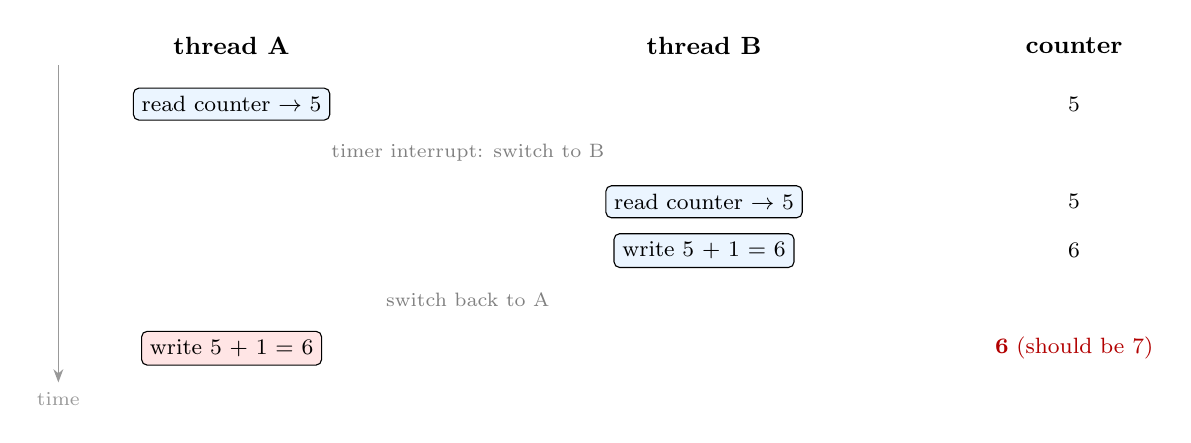
\begin{tikzpicture}[font=\footnotesize, x=1cm, y=0.62cm, box/.style={draw,rounded corners=2pt,inner sep=3pt,align=center}]
  \node[font=\small\bfseries] at (2.5,7.2) {thread A};
  \node[font=\small\bfseries] at (8.5,7.2) {thread B};
  \node[font=\small\bfseries] at (13.2,7.2) {counter};
  \node[box,fill=newbg] at (2.5,6) {read counter $\to$ 5};
  \node[black!50] at (5.5,5) {\scriptsize timer interrupt: switch to B};
  \node[box,fill=newbg] at (8.5,4) {read counter $\to$ 5};
  \node[box,fill=newbg] at (8.5,3) {write 5 + 1 = 6};
  \node[black!50] at (5.5,2) {\scriptsize switch back to A};
  \node[box,fill=red!10] at (2.5,1) {write 5 + 1 = 6};
  \node at (13.2,6) {5}; \node at (13.2,4) {5}; \node at (13.2,3) {6}; \node[red!70!black] at (13.2,1) {\textbf{6} (should be 7)};
  \draw[-{Stealth},black!40] (0.3,6.8) -- (0.3,0.3) node[below] {\scriptsize time};
\end{tikzpicture}
\end{center}
Both threads did ``+1'', but the counter only grew by one. The test does this 80\,000 times with 4
threads -- without a working lock, many increments get lost.

\subsection*{Picture 2 -- the fix: a lock around the critical section}

\begin{center}
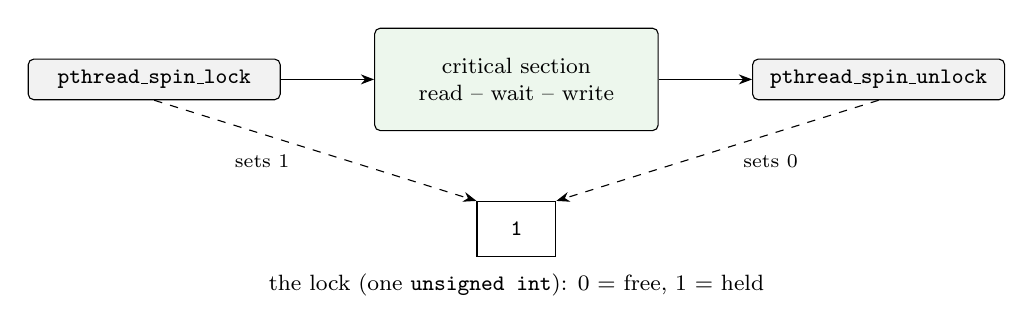
\begin{tikzpicture}[font=\footnotesize, box/.style={draw,rounded corners=2pt,inner sep=4pt,align=center}]
  \node[box,fill=black!5,minimum width=3.2cm] (l) at (0,0) {\code{pthread\_spin\_lock}};
  \node[box,fill=keybg,minimum width=3.6cm,minimum height=1.3cm] (c) at (4.6,0) {critical section\\read -- wait -- write};
  \node[box,fill=black!5,minimum width=3.2cm] (u) at (9.2,0) {\code{pthread\_spin\_unlock}};
  \draw[-{Stealth}] (l) -- (c); \draw[-{Stealth}] (c) -- (u);
  \node[draw,minimum width=1cm,minimum height=0.7cm,fill=white] (v) at (4.6,-1.9) {\code{1}};
  \node[below,align=center] at (4.6,-2.35) {the lock (one \code{unsigned int}): 0 = free, 1 = held};
  \draw[-{Stealth},dashed] (l.south) -- node[pos=0.45,below left] {\scriptsize sets 1} (v.north west);
  \draw[-{Stealth},dashed] (u.south) -- node[pos=0.45,below right] {\scriptsize sets 0} (v.north east);
\end{tikzpicture}
\end{center}
Only one thread at a time can be between \code{lock} and \code{unlock}. The others wait at
\code{lock} until the holder calls \code{unlock}.

\subsection*{Picture 3 -- why ``check, then set'' is not enough, and test-and-set is}

\begin{center}
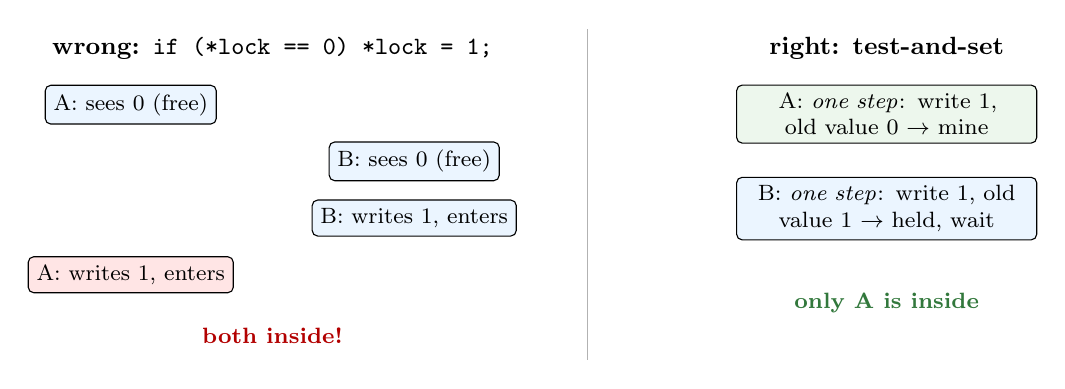
\begin{tikzpicture}[font=\footnotesize, x=1cm, y=0.6cm, box/.style={draw,rounded corners=2pt,inner sep=3pt,align=center}]
  \node[font=\small\bfseries] at (3.6,7.0) {wrong: \code{if (*lock == 0) *lock = 1;}};
  \node[box,fill=newbg] at (1.8,5.8) {A: sees 0 (free)};
  \node[box,fill=newbg] at (5.4,4.6) {B: sees 0 (free)};
  \node[box,fill=newbg] at (5.4,3.4) {B: writes 1, enters};
  \node[box,fill=red!10] at (1.8,2.2) {A: writes 1, enters};
  \node[red!70!black,align=center] at (3.6,0.9) {\textbf{both inside!}};
  \node[font=\small\bfseries] at (11.4,7.0) {right: test-and-set};
  \node[box,fill=keybg,text width=3.6cm] at (11.4,5.6) {A: \emph{one step}: write 1, old value 0 $\to$ mine};
  \node[box,fill=newbg,text width=3.6cm] at (11.4,3.6) {B: \emph{one step}: write 1, old value 1 $\to$ held, wait};
  \node[keyrule,align=center] at (11.4,1.6) {\textbf{only A is inside}};
  \draw[black!30] (7.6,0.4) -- (7.6,7.4);
\end{tikzpicture}
\end{center}
On the left, a thread switch can happen \emph{between} ``look'' and ``write''. On the right, looking
and writing are one indivisible step -- there is no ``between''.

\subsection*{Picture 4 -- why wait with \code{sched\_yield}}

\begin{center}
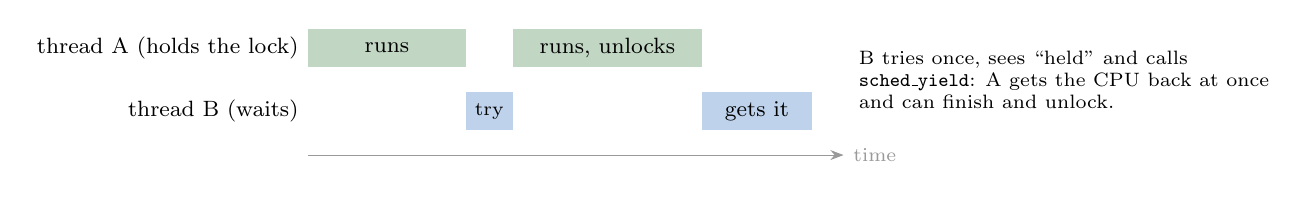
\begin{tikzpicture}[font=\footnotesize, x=1cm, y=0.8cm]
  \node[left] at (0,2) {thread A (holds the lock)};
  \node[left] at (0,1) {thread B (waits)};
  \fill[keyrule!30] (0,1.7) rectangle (2,2.3);  \node at (1,2) {runs};
  \fill[newrule!30] (2,0.7) rectangle (2.6,1.3); \node at (2.3,1) {\scriptsize try};
  \fill[keyrule!30] (2.6,1.7) rectangle (5,2.3); \node at (3.8,2) {runs, unlocks};
  \fill[newrule!30] (5,0.7) rectangle (6.4,1.3); \node at (5.7,1) {gets it};
  \draw[-{Stealth},black!40] (0,0.3) -- (6.8,0.3) node[right] {\scriptsize time};
  \node[align=left,font=\scriptsize] at (9.6,1.5) {B tries once, sees ``held'' and calls\\
    \code{sched\_yield}: A gets the CPU back at once\\and can finish and unlock.};
\end{tikzpicture}
\end{center}
Without \code{sched\_yield}, B would keep trying for its whole time slice -- while A, the only thread
that can unlock, does not get the CPU (SWEB runs on one CPU). That wastes time, it does not break
the lock.

% =====================================================================================
\clearpage
\section*{The goal (level 1)}

\begin{lstlisting}[language={},basicstyle=\ttfamily\footnotesize]
Name:         pthread_spin_init/destroy/lock/trylock/unlock,
              pthread_mutex_init/destroy/lock/unlock (pthread.h - the stubs exist)
Description:  A lock is one unsigned int (0 = free, 1 = held). lock waits until the lock
              is free and takes it; trylock takes it only if it is free; unlock frees it.
              While waiting, give the CPU to the other threads (sched_yield) - the holder
              needs it to unlock. The mutex may behave exactly like the spinlock.
Return Value: 0, or -1 (NULL; trylock: the lock is held)
\end{lstlisting}

In your team's \file{pthread.h}: \code{typedef unsigned int pthread\_spinlock\_t;} and
\code{typedef unsigned int pthread\_mutex\_t;} -- both are just one number, so the mutex functions
can simply call the spinlock functions.

\section*{What each function does, in simple terms}

The lock is \textbf{one number}: \code{0} = free, \code{1} = taken.

{\small
\begin{tabular}{@{}L{5.2cm} L{10.2cm}@{}}
\toprule
\textbf{Function} & \textbf{What it does}\\\midrule
\code{pthread\_spin\_init(lock, \ldots)} & \textbf{Prepare} the lock: set it to \code{0} (free).\\
\code{pthread\_spin\_destroy(lock)} & \textbf{Throw} the lock away. There is nothing to clean up, so it just says ``OK'' (\code{0}).\\
\code{pthread\_spin\_lock(lock)} & \textbf{Take} the lock. If someone else has it, \textbf{wait} (let the others run) and try again until you get it.\\
\code{pthread\_spin\_trylock(lock)} & \textbf{Try once} to take the lock. Free $\to$ take it (\code{0}). Taken $\to$ \textbf{do not wait}, give up right away (\code{-1}).\\
\code{pthread\_spin\_unlock(lock)} & \textbf{Give} the lock back: set it to \code{0}, so the next one can take it.\\
\code{pthread\_mutex\_init} & the same as \code{spin\_init} (it just calls it)\\
\code{pthread\_mutex\_destroy} & the same as \code{spin\_destroy}\\
\code{pthread\_mutex\_lock} & the same as \code{spin\_lock}\\
\code{pthread\_mutex\_unlock} & the same as \code{spin\_unlock}\\
\bottomrule
\end{tabular}}

\smallskip
\textbf{Every function also checks:} if you pass \code{NULL} (no lock at all), return \code{-1} instead of crashing.

\subsection*{How the test uses them}

\begin{lstlisting}[language={},basicstyle=\ttfamily\small]
init     ->  lock = 0
lock     ->  lock = 1   (I'm in)
   counter + 1          (only I can do this now)
unlock   ->  lock = 0   (the next one can go in)
\end{lstlisting}

All 4 threads do this 20\,000 times. Because only one is ever ``in'', no ``+1'' is lost, and the counter
ends at exactly 80\,000.

\section*{The order: 8 steps, two files}

{\small
\begin{tabular}{@{}l L{6.2cm} L{3.6cm} L{5.0cm}@{}}
\toprule
\# & What & File & Why\\\midrule
1 & declare the 5 spinlock functions & \file{pthread.h} & they exist in \file{pthread.c} but are not declared -- the test would not compile\\
2 & include \file{sched.h} & \file{pthread.c} & for \code{sched\_yield}\\
3 & \code{pthread\_spin\_init} & \file{pthread.c} & a new lock starts free\\
4 & \code{pthread\_spin\_destroy} & \file{pthread.c} & nothing to free\\
5 & \code{pthread\_spin\_lock} & \file{pthread.c} & \textbf{the core: test-and-set + yield}\\
6 & \code{pthread\_spin\_trylock} & \file{pthread.c} & test-and-set once\\
7 & \code{pthread\_spin\_unlock} & \file{pthread.c} & set it back to 0\\
8 & the four \code{pthread\_mutex\_\ldots} & \file{pthread.c} & call the spinlock functions\\
\bottomrule
\end{tabular}}

% =====================================================================================
\section{Declare the spinlock functions \hfill {\normalsize\file{userspace/libc/include/pthread.h}}}

After the declaration of \code{pthread\_cond\_wait} (around line 61):

\begin{lstlisting}
extern int pthread_spin_init(pthread_spinlock_t *lock, int pshared);
extern int pthread_spin_destroy(pthread_spinlock_t *lock);
extern int pthread_spin_lock(pthread_spinlock_t *lock);
extern int pthread_spin_trylock(pthread_spinlock_t *lock);
extern int pthread_spin_unlock(pthread_spinlock_t *lock);
\end{lstlisting}

\begin{itemize}
  \item The functions are already \emph{defined} (as stubs) in \file{pthread.c}, but the header does not
        \emph{declare} them. The test includes \file{pthread.h}; SWEB compiles user programs with
        \code{-Werror=implicit-function-declaration} -- calling an undeclared function is an error.
  \item Copy the signatures exactly from the stubs in \file{pthread.c} (a header and its \file{.c} must agree).
  \item \code{extern}: ``this function exists somewhere else'' -- the usual style of this header.
\end{itemize}

\begin{infobox}[title={How would I know that?},fonttitle=\bfseries\small,coltitle=white,colbacktitle=newrule]
You do not have to guess -- two quick checks tell you, and both work for \emph{every} type-U task:
\begin{enumerate}
  \item \textbf{Build first, before writing anything:} \code{task start a1-15}, then \code{task test}. The
        build stops with \code{error: implicit declaration of function 'pthread\_spin\_init'} (and the
        same for the others) -- the compiler names exactly the functions that are not declared.
  \item \textbf{Look for the declaration yourself:} \code{grep -n "pthread\_spin" userspace/libc/include/pthread.h}
        finds only the \code{typedef}, no function -- while
        \code{grep -n "pthread\_spin" userspace/libc/src/pthread.c} finds all five stubs.
\end{enumerate}
The rule behind it: a program can only call a library function if a \textbf{header} declares it. The
stub in the \file{.c} file is the \emph{definition} (the code); the line in the \file{.h} file is the
\emph{declaration} (``this function exists, with these parameters''). A stub without a declaration
is invisible to the test program.
\end{infobox}

\done{Five declarations in \file{pthread.h}.}

% =====================================================================================
\section{Include \code{sched.h} \hfill {\normalsize\file{userspace/libc/src/pthread.c}}}

At the top, next to the other includes:

\begin{lstlisting}
#include "sched.h"
\end{lstlisting}

\code{sched\_yield} is declared in \file{sched.h}. Without the include, its call in step 5 is again an
``implicit declaration'' error.

\done{One line at the top of \file{pthread.c}.}

% =====================================================================================
\section{\code{pthread\_spin\_init} \hfill {\normalsize\file{pthread.c}}}

Replace the body of the stub:

\begin{lstlisting}[numbers=left,numberstyle=\tiny\color{headgray}]
int pthread_spin_init(pthread_spinlock_t *lock, int pshared)
{
  (void) pshared;
  if (!lock)
    return -1;
  *lock = 0;
  return 0;
}
\end{lstlisting}

\begin{description}
  \item[Line 3.] \code{pshared} (``shared between processes?'') is not needed here. \code{(void)} tells the
        compiler (and the reader) ``unused on purpose''.
  \item[Lines 4--5.] A \code{NULL} pointer is not a lock: return \code{-1} instead of crashing on \code{*lock}.
  \item[Line 6.] \code{lock} is a \emph{pointer} to the lock variable; \code{*lock} is the variable itself.
        A new lock starts \textbf{free} = 0.
  \item[Line 7.] Success.
\end{description}

\done{\code{init} sets the lock to 0.}

% =====================================================================================
\section{\code{pthread\_spin\_destroy} \hfill {\normalsize\file{pthread.c}}}

\begin{lstlisting}
int pthread_spin_destroy(pthread_spinlock_t *lock)
{
  if (!lock)
    return -1;
  return 0;
}
\end{lstlisting}

The lock is one number inside the caller's memory -- there is nothing to free. Only \code{NULL} is an error.

\done{\code{destroy} returns 0 for a real lock.}

% =====================================================================================
\section{\code{pthread\_spin\_lock} -- the core \hfill {\normalsize\file{pthread.c}}}

\begin{lstlisting}[numbers=left,numberstyle=\tiny\color{headgray}]
int pthread_spin_lock(pthread_spinlock_t *lock)
{
  if (!lock)
    return -1;
  while (__sync_lock_test_and_set(lock, 1))
    sched_yield();
  return 0;
}
\end{lstlisting}

\begin{description}
  \item[Lines 3--4.] \code{NULL} check, as in \code{init} (the test checks it).
  \item[Line 5 -- test-and-set.] \code{\_\_sync\_lock\_test\_and\_set(lock, 1)} is a compiler built-in. It
        writes 1 into \code{*lock} and returns the value that was there \textbf{before} -- in \textbf{one
        indivisible step} (the CPU instruction \code{xchg}). So:
        \begin{itemize}
          \item returns 0 $\Rightarrow$ the lock was free, and we just made it 1 $\Rightarrow$ it is ours,
                the \code{while} ends;
          \item returns 1 $\Rightarrow$ someone else holds it (writing 1 again changed nothing)
                $\Rightarrow$ loop again.
        \end{itemize}
        Why not \code{while (*lock) \{\}} followed by \code{*lock = 1}? See picture 3: a thread switch
        between the look and the write lets two threads in.
  \item[Line 6 -- \code{sched\_yield}.] The lock is held: give the CPU away so the holder can run and
        unlock (picture 4). Then the loop tries again.
  \item[Line 7.] We hold the lock.
\end{description}

\begin{trapbox}
The test \emph{cannot} prove that your lock is atomic: the naive ``look, then write'' version usually
passes too, because the timer rarely hits exactly between the two instructions. Such bugs survive
testing -- in the interview the tutor asks \emph{why} yours is correct. Answer: test-and-set is one
indivisible step.
\end{trapbox}

\done{\code{lock} loops with test-and-set and yields while the lock is held.}

% =====================================================================================
\section{\code{pthread\_spin\_trylock} \hfill {\normalsize\file{pthread.c}}}

\begin{lstlisting}[numbers=left,numberstyle=\tiny\color{headgray}]
int pthread_spin_trylock(pthread_spinlock_t *lock)
{
  if (!lock)
    return -1;
  if (__sync_lock_test_and_set(lock, 1) != 0)
    return -1;
  return 0;
}
\end{lstlisting}

\begin{description}
  \item[Line 5.] The same test-and-set as in \code{lock}, but only \textbf{once}, no loop. Old value 1
        $\Rightarrow$ held by someone else $\Rightarrow$ \code{-1} at once (line 6). We wrote 1 into a lock
        that was already 1 -- nothing changed, so there is nothing to undo.
  \item[Line 7.] Old value 0 $\Rightarrow$ it was free and is ours now.
\end{description}

\done{\code{trylock} succeeds on a free lock and fails at once on a held one.}

% =====================================================================================
\section{\code{pthread\_spin\_unlock} \hfill {\normalsize\file{pthread.c}}}

\begin{lstlisting}[numbers=left,numberstyle=\tiny\color{headgray}]
int pthread_spin_unlock(pthread_spinlock_t *lock)
{
  if (!lock)
    return -1;
  __sync_lock_release(lock);
  return 0;
}
\end{lstlisting}

\begin{description}
  \item[Line 5.] \code{\_\_sync\_lock\_release} writes 0 = free. Why not just \code{*lock = 0}? The built-in
        also forbids the compiler (and CPU) to move writes of the critical section \emph{after} the
        unlock -- otherwise the next thread could see the lock free before the counter is written.
        (On x86, \code{*lock = 0} would usually work too; the built-in is the safe, portable way.)
\end{description}

\done{\code{unlock} sets the lock back to 0.}

% =====================================================================================
\section{The mutex functions \hfill {\normalsize\file{pthread.c}}}

The card says the mutex may behave exactly like the spinlock. Both types are \code{unsigned int}, so
each mutex function just calls its spinlock partner:

\begin{lstlisting}
int pthread_mutex_init(pthread_mutex_t *mutex, const pthread_mutexattr_t *attr)
{
  (void) attr;
  return pthread_spin_init(mutex, 0);
}

int pthread_mutex_destroy(pthread_mutex_t *mutex)  { return pthread_spin_destroy(mutex); }
int pthread_mutex_lock(pthread_mutex_t *mutex)     { return pthread_spin_lock(mutex); }
int pthread_mutex_unlock(pthread_mutex_t *mutex)   { return pthread_spin_unlock(mutex); }
\end{lstlisting}

\begin{itemize}
  \item Write each one in the existing stub (keep the stubs' line layout -- the short form above only
        saves space here). No duplicated logic: if the spinlock is right, the mutex is right.
  \item \code{attr} (mutex options) is not needed: \code{(void) attr;} marks it as unused on purpose.
  \item The \code{NULL} check comes for free: \code{pthread\_mutex\_lock(0)} calls
        \code{pthread\_spin\_lock(0)}, which returns \code{-1}.
  \item The mutex functions are \emph{defined above} the spinlock functions in \file{pthread.c} -- that
        is fine because step 1 declared them in \file{pthread.h}, which \file{pthread.c} includes.
\end{itemize}

\done{\code{task test} shows \textbf{7 of 7 passed}.}

% =====================================================================================
\section*{The test -- what each check means}

{\small
\begin{tabular}{@{}L{6.4cm} L{8.8cm}@{}}
\toprule
\textbf{Check} & \textbf{Which step makes it pass}\\\midrule
init & steps 3 + 8 (\code{mutex\_init} calls \code{spin\_init})\\
trylock on a free lock & step 6: old value 0 $\to$ 0\\
trylock on a held lock fails & step 6: old value 1 $\to$ \code{-1}\\
free again after unlock & step 7 sets 0, step 6 takes it again\\
spinlock: no increment lost & step 5: 4 threads $\times$ 20\,000 increments = 80\,000\\
mutex: no increment lost & step 8: the same with the mutex functions\\
NULL rejected & the \code{if (!lock)} in steps 5 and 8\\
\bottomrule
\end{tabular}}

\section*{Say it in three sentences}

\begin{keybox}[title={Remember}]
\begin{itemize}
  \item A lock is one number: 0 = free, 1 = held; \textbf{lock} takes it, \textbf{unlock} sets it back to 0.
  \item Taking it must be \textbf{one indivisible step} (test-and-set = \code{xchg}): write 1, look at the
        old value -- 0 means ``mine''.
  \item While it is held, \textbf{yield} the CPU so the holder can run and unlock.
\end{itemize}
\end{keybox}

\section*{Questions a tutor might ask}

{\small
\begin{tabular}{@{}L{6.4cm} L{8.8cm}@{}}
\toprule
\textbf{Question} & \textbf{Short answer}\\\midrule
Why not \code{if (*lock == 0) *lock = 1;}? & a thread switch between the check and the write lets two threads in (picture 3)\\
What does \code{\_\_sync\_lock\_test\_and\_set} return? & the \emph{old} value; it writes the new one in the same step\\
Which CPU instruction is behind it? & \code{xchg} -- exchange a register with memory, atomic on x86\\
Why \code{sched\_yield} in the loop? & one CPU: the holder needs the CPU to unlock; spinning wastes the time slice\\
Does the test prove the lock is correct? & no -- the naive version usually passes too; the argument is atomicity\\
Spinlock vs.\ real mutex? & spinlock: keeps trying; real mutex: sleeps in the kernel (wait queue), woken by unlock\\
When is spinning OK? & several CPUs and very short critical sections; on one CPU it only makes sense with yield\\
Why \code{\_\_sync\_lock\_release} and not \code{*lock = 0}? & keeps the compiler/CPU from moving critical-section writes after the unlock\\
What happens if a thread calls \code{lock} twice? & it waits for itself forever -- a deadlock (this lock is not recursive)\\
What about the kernel's locks? & the kernel has its own \code{SpinLock} and \code{Mutex} (\code{Mutex} sleeps) -- user programs cannot use them directly\\
\bottomrule
\end{tabular}}

\end{document}
